\begin{figure}[htbp]
    \centering
    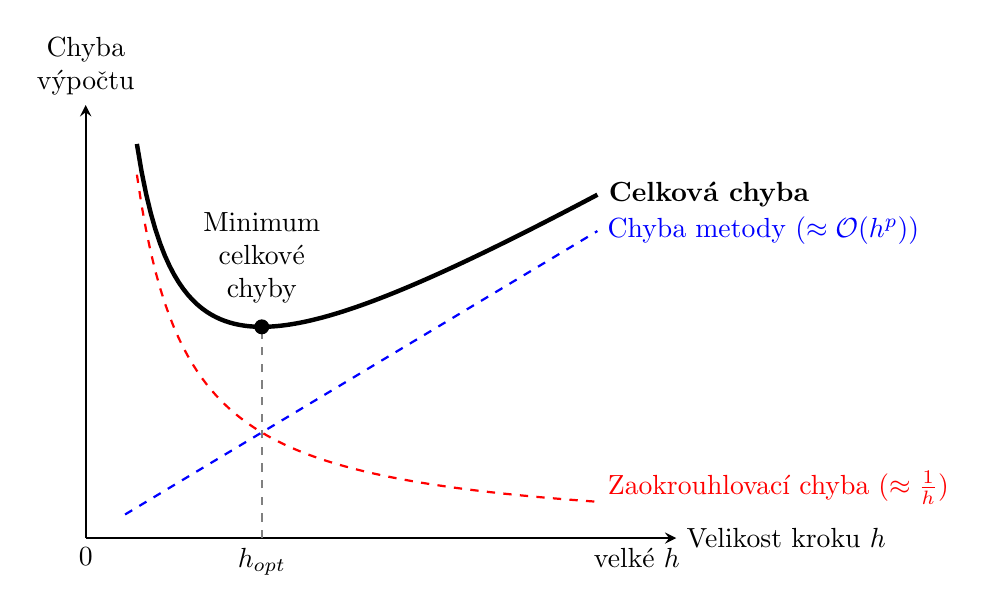
\begin{tikzpicture}[>=stealth]
        % Osy
        \draw[->, thick] (0,0) -- (7.5,0) node[right, align=center] {Velikost kroku $h$};
        \draw[->, thick] (0,0) -- (0,5.5) node[above, align=center] {Chyba\\výpočtu};
        
        % Osa logaritmická - naznačení směru k nule
        \node[below] at (0,0) {$0$};
        \node[below] at (7,0) {velké $h$};
        
        % Chyba metody (analytická chyba) - roste s rostoucím h
        % Vykreslíme jako lineární/polynomiální funkci (např. y = 0.6 * x)
        \draw[domain=0.5:6.5, color=blue, thick, dashed, samples=100] 
            plot (\x, {0.6*\x}) node[right] {\textcolor{blue}{Chyba metody ($\approx \mathcal{O}(h^p)$)}};
            
        % Zaokrouhlovací chyba (numerická chyba) - roste s klesajícím h
        % Vykreslíme jako nepřímou úměru (např. y = 3 / x)
        \draw[domain=0.65:6.5, color=red, thick, dashed, samples=100] 
            plot (\x, {3/\x}) node[right, yshift=5pt] {\textcolor{red}{Zaokrouhlovací chyba ($\approx \frac{1}{h}$)}};
            
        % Celková chyba = Chyba metody + Zaokrouhlovací chyba
        \draw[domain=0.65:6.5, color=black, ultra thick, samples=100] 
            plot (\x, {0.6*\x + 3/\x}) node[right, font=\bfseries] {Celková chyba};
            
        % Nalezení minima (optimálního h)
        % Minimum funkce f(x) = 0.6x + 3/x je v bodě x = sqrt(3/0.6) = sqrt(5) ≈ 2.236
        % y = 0.6*2.236 + 3/2.236 = 1.341 + 1.341 = 2.683
        \coordinate (Opt) at (2.236, 2.683);
        
        % Vyznačení optimálního bodu
        \draw[dashed, gray, thick] (2.236, 0) -- (Opt);
        \filldraw[black] (Opt) circle (2.5pt) node[above=5pt, align=center] {Minimum\\celkové\\chyby};
        \node[below, font=\bfseries] at (2.236, 0) {$h_{opt}$};
        
    \end{tikzpicture}
    \caption{Závislost celkové chyby numerického derivování na velikosti kroku $h$. Při příliš malém kroku dominuje zaokrouhlovací chyba počítače (červená křivka), při příliš velkém kroku je metoda matematicky nepřesná (modrá křivka). Naším cílem je najít optimální krok $h_{opt}$.}
    \label{fig:optimalni_h}
\end{figure}